\section{Eine Einführung in die IT für Arbeitsplätze geben}
\subsection{Eine Einführung in Grundfunktionen des Computers geben}
    \vspace{0.5em}
    \begin{tcolorbox}[width=9cm, center, title=EVA-Grundprinzip der Datenverarbeitung, coltitle=white, colframe=orange, colback=white!60!orange]
        \begin{itemize}
            \item[E =] Eingabe
            \item[V =] Verarbeitung
            \item[A =] Ausgabe
        \end{itemize}
    \end{tcolorbox}
    \vspace{-0.5em}
    \begin{figure}[h]
        \centering
        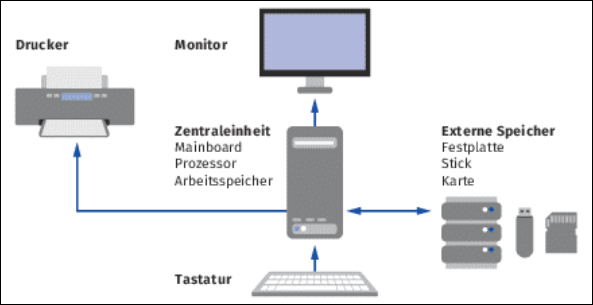
\includegraphics[width=0.7\textwidth]{./images/2.1.1_konfiguration.png}
        \caption{EVA-Prinzip Beispiel}\label{fig:EVA-Prinzip}
    \end{figure}
    \vspace{-0.5em}
    \begin{tcolorbox}[width=13cm, center, title=Konfiguration, coltitle=white, colframe=white!20!blue, colback=white!80!blue]
        Bezeichnung für abgestimmte Zusammenstellung von Hardware und Software auf Nutzungszweck des Kunden.
    \end{tcolorbox}
    \vspace{0.25em}
\subsection{Bedeutende Entwicklungsschritte in der Computertechnik}
    \vspace{0.5em}
    \begin{itemize}[leftmargin=3cm]
        \item[1980er:] IBM, 8Bit Prozessor, 64KB RAM
        \item[1990er:] Open Source, Internet, Google
        \item[2000er:] Open Office, Facebook
        \item[2020er:] KI, 64Bit Prozessor, 64GB+ RAM
        \item[2030er:] Quantencomputer
    \end{itemize}

\newpage
\subsection{Entwicklungstrends präsentieren}
    \vspace{-0.5em}
    \begin{figure}[h]
        \centering
        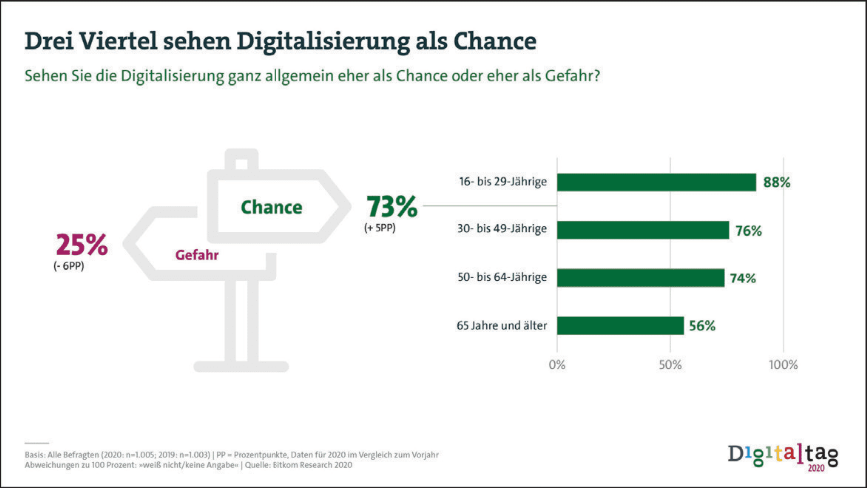
\includegraphics[width=0.7\textwidth]{./images/2.1.3_entwicklungstrend-digitalisierung.png}
        \caption{Entwicklungstrend zur Digitalisierung}\label{fig:Entwicklungstrend_Digitalisierung}
    \end{figure}
    \vspace{-0.5em}
\subsection{Komponentenhersteller und Systemarchitekturen präsentieren}
    \begin{subindent}
        Wichtige Hersteller in der heutigen Zeit:
    \end{subindent}
    \vspace{-0.5em}
    \begin{itemize}[leftmargin=2.5cm]
        \item Intel (Prozessor Marktführer)
        \item AMD (Konkurrent zu Intel)
        \item NVIDIA (Größter Grafikkartenentwickler)
        \item ARM (Prozessorarchitektur)
        \item Apple
        \item Microsoft (Betriebssystem Marktführer)
    \end{itemize}
    \vspace{0.5em}
    \begin{tcolorbox}[width=15cm, center, title=Kompatibilität, coltitle=white, colframe=white!20!blue, colback=white!80!blue]
        Bezeichnung für Verträglichkeit von Komponenten zeinander.
        \begin{itemize}[labelsep=1em, align=parleft, leftmargin=*, widest=Abwärtskompabilität, itemsep=0em]
            \item[Aufwärtskompabilität:] Vorgängerversionen funktionieren mit Nachfolgeversionen
            \item[Abwärtskompabilität: ] neuere Komponenten funktionieren mit Vorgängerversionen
        \end{itemize}
    \end{tcolorbox}
\subsection*{Reflexion Kapitel 2.1}
\addcontentsline{toc}{subsection}{Reflexion Kapitel 2.1}
    \begin{refindent}
        Grundlage zur Verbindung der einzelnen Komponenten eines Computers erlernt (EVA-Prinzip, Konfiguration und Kompatibilität).
        Ebenso ein grobes Wissen über die Entwicklung der IT erlangt, mit möglichen zukünftigen Entwicklungen.
        Verschiedene Hersteller kennengelernt, die einen Großteil des Marktes ausmachen.
    \end{refindent}